\chapter{Gegenüberstellung}
\thispagestyle{fancy}
\section{Planung}

Das Thema Planung wird unter folgenden fünf Aspekten betrachtet:
\begin{enumerate}
\item Release-Planung
\item Priorisierung
\item Planungssicherheit
\item Planungsaufwands
\item Nachvollziehbarkeit
\end{enumerate}

\subsection{Release-Planung}

{\Large Scrum:} \cite{planningReleaseScrum} \medskip

Der Release-Plan ist ein höhergestellter Plan, der mehrere Sprint beinhaltet und während der Release-Planung festgelegt wird. Der Plan definiert welche Features umgesetzt werden und wann diese erfüllt sind. Er dient auch dazu, den Fortschritt innerhalb des Projekts verfolgen zu können. Es können mehrere Releases während des Projekt geplant werden, oder einfach ein finales Release am Ende des Projekts. \medskip

Um eine Relaese-Planung durchführen zu können muss folgendes bekannt sein:
\begin{itemize}
\item Ein priorisiertes Scrum-Backlog
\item Die Ressourcen des Scrum-Teams
\item Zielerfüllungsbedingungen
\end{itemize}
Ein Release-Plan kann Termin- oder Feature-geführt sein.\smallskip

Bei Termin-geführten Projekten wird spezifiziert, welche Features bis zu einem bestimmten Termin erfüllt werden können.\smallskip
Kommt es bei einem Termin-geführten Projekt zu Verzögerungen, so muss gegebenenfalls der Termin angepasst werden. Dies muss in Abstimmung mit dem Kunden gemacht werden.

Bei Feature-geführten Projekten wird spezifiziert , bis zu welchem Termin das Features erfüllt ist. Kommt es bei Feature-geführten Projekten zu Verzögerungen, so muss zusammen mit dem Kunden besprochen werden, welche Features gegebenenfalls weggelassen werden können entsprechend angepasst werden müssen.\smallskip

Wie der Backlog ist auch der Release-Plan bei Scrum nicht statisch. Dieser kann sich mit dem Backlog ändern oder auch nach jedem Sprint wieder diskutiert und überarbeitet werden.
\bigskip 

{\Large DAD:} \cite{planningReleaseDad} \medskip

In DAD wird die Release Planung initial in der Inception Phase gemacht. Der Leitfaden empfiehlt für die Releaseplanung folgende sechs Fragen zu beantworten.
\begin{itemize}
	\item Wer wird an der Planung beteiligt sein?
	\item Was ist der Umfang unseres Planungsaufwands?
	\item Was ist unsere Gesamtstrategie, die diesen Plan vorantreibt?
    \item Wie detailliert sollte unser Plan sein?
    \item Welche Kadenzen wird das Team annehmen?
    \item Welchen Ansatz zur Schätzung werden wir wählen?
\end{itemize}
Damit soll sichergestellt werden, dass grundlegende Managementfragen gegenüber den Stakeholder beantwortet sind. Zudem wird erreicht, dass eine durchführbare Strategie besteht und zwischen Stakeholder und Delivery Team ein gemeinsames Verständnis existiert.


\subsection{Priorisierung}

{\Large Scrum:} \cite{planningPrioScrum} \medskip

Das Scrum-Team priorisiert zusammen mit dem Product-Owner die Tasks/Stories aus dem Scurm-Backlog. Wichtig dabei ist, dass nicht nur priorisiert, sondern dass auch sortiert werden muss. Beim Sortieren wird auch die Reihenfolge von Abläufen berücksichtigt. Die Priorisierung geht mit der Sortierung Hand in Hand. \smallskip

Weiter achtet Scrum auch darauf, dass die wertvollsten Inkremente frühstmöglich umgesetzt werden.\bigskip 

{\Large DAD:} \cite{planningPrioDad} \medskip

Die Priorisierung bei DAD verhält sich ähnlich wie die Release-Planung. Grundsätzlich gilt wieder das Rolling-Wave-Modell. Dass heisst, dass höher priorisierte Features detaillierter spezifiziert werden und tief priorisierte nur grob. Die Priorisierung kann zu jederzeit wieder angepasst werden.


\subsection{Planungsumfang}

{\Large Scrum:} \medskip

In Scrum betrifft der Umfang immer direkt das Produkt. Der Scope beinhaltet Features ausgedrückt z.B. als User Stories. Diese sind Im Scrum-Backlog abgelegt und verwaltet.
\bigskip 

{\Large DAD:} \cite{planningScopeDad} \medskip

DAD geht hier einen Schritt weiter und definiert nicht nur Features sondern sogenannte Working-Items. Bei denen werden auch nicht-funktionale Anforderungen definiert wie z.B. Schulungen, Ferien, Unterstützung anderer Teams usw.	


\subsection{Planungsaufwand}

{\Large Scrum:} \medskip

Der Planungsaufwand von Scrum ist relativ gering und ist eigentlich im iterierenden Prozess von Scrum bereits integriert. Die Planung wird bei Scrum vor jedem Sprint im sogenannten Sprint Planning gemacht. Dabei werden die zu erledigenden Items definiert. Der Umfang des Sprints wird vom ganzen Team bestätigt.\bigskip 

{\Large DAD:} \medskip

Initial ist der Planungsaufwand bei DAD hoch. Man muss nebst der eigentlichen Planung des Produkts auch diverse Analysen von Ist-Zuständen bezüglich Ressourcen und Zuständen innerhalb des Unternehmens machen um die Rahmenbedingungen für das Projekt zu legen. Während der Construction Phase ist der Planungsaufwand anlog jenem von Scrum.


\subsection{Risikomanagement}

{\Large Scrum:} \medskip

Bei Scrum wird das Risikomanagement hauptsächlich durch die Kommunikation zwischen dem Kunden und Team geführt. Dies geht über den Product Owner. Dabei muss der Kunde durch seinen stetigen Einfluss mögliche Risiken ausschliessen können. Er kann dies mittels Akzeptanzkriterien beeinflussen.\newline
Aus Team-interner Sicht ist die Definition of Done das Kontrollinstrument um Qualität aber auch Vollständigkeit sicherzustellen.
Als weiteres Instrument dient die Review am Ende jedes Sprints. An jener wird dem Kunde die umgsetzten Items präsentiert. Hier kann der Kunde oder der Product Owner Einfluss bzw. Missverständnisse aufdecken und klären.

\bigskip 

{\Large DAD:} \medskip

Um das Risiko von Fehlkommunikation zu verringern werden bei DAD gegenüber Scrum leichte Meilenstein eingeführt, bei denen ein Abgleich mit dem Kunden stattfindet. \medskip

Weiter sieht DAD die Planung von festen Releases vor. Damit soll regelmässig Software zur Verfügung gestellt werden um ein Feedback des Kunden zu erhalten und frühzeitig festzustellen, ob man die Anforderungen so erfüllen kann. Dies ist gleich wie bei Scrum.

\section{Zuständigkeit}
\subsection{Rollen}
{\Large Scrum:} \medskip

In Scrum gibt es drei Rollen. Den Scrum Master, den Product Owner und die Team Member. 
\begin{figure}[H]
	\centering
	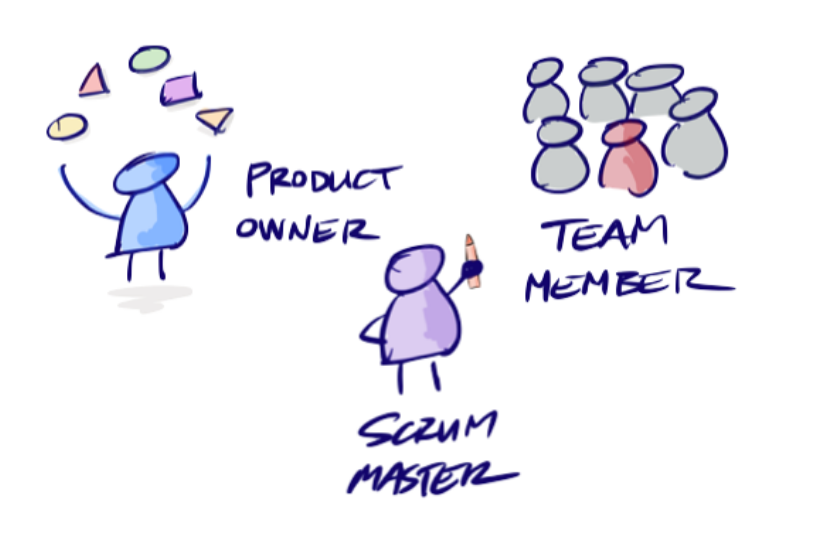
\includegraphics[scale=0.8]{scrum_roles}
	\caption{Scrum Rollen}
	\label{fig:scrumrollen}
\end{figure}

Der \textbf{Product Owner} ist die Ansprechsperson für Kunden und Stakeholder. Er nimmt die Anforderungen entgegen, priorisiert diese und gibt diese an das Team weiter. Der Product Owner kann aber auch direkt der Kunde sein. In beiden Fällen vertritt er aber die fachliche Sicht, beurteilt die Qualität, Usability und Performance. \medskip

Der \textbf{Scrum Master} dient dem Scrum Team um die gewünschte Performance zu erreichen. Er ist verantwortlich, dass der Prozess zielgerichtet ausgeführt werden kann. Er nimmt sich Problemen, sogenannte Impediments, an und löst diese - mit oder ohne Team. Der Scrum Master überwacht TODO zudem den Fortschritt, organisiert die Scrum Zeremonien - Retrospektive, Review-Meeting, Daily Standups - und sorgt für den Informationsfluss zwischen Team und Product Owner. Er ist sozusagen die gute Seele des Teams. \medskip

Das \textbf{Scrum Team}, oder kurz Team, ist das zentrale Element im Scrum Prozess. Es setzt die Anforderungen um. In Scurm besteht ein Team aus fünf bis zehn Personen. Grössere Teams sollten in mehrere unabhängige Teams aufgetrennt werden. Sehr wichtig bei Scrum ist, dass das Team selbstorganisiert. Es bestimmt schlussendlich selbst, welche Anforderungen es im Sprint umsetzten will. Dabei beachtet es, dass es am Ende jedes Sprints ein «Increment of  Potentially Shippable Functionality» liefert. In einem Scrum Team sind immer die Disziplinen vorhanden, welche es für das Erreichen des Ziels benötigt.
\bigskip 

{\Large DAD:} \medskip

Im Gegensatz zu Scrum werden in DAD zusätzliche Rollen definiert. In DAD werden einzelne Zuständigkeiten explizit aufgeführt, welche in Scrum im Team vereint werden. DAD verwendet gewisse Rollen aus dem Agilen Manifest (Team Member und Product Owner). DAD unterscheidet hierbei primäre und unterstützende Rollen. Zu den primären Rollen zählen Team Lead, Product Owner, Team Member, Archictecture Owner und Stakeholder. Zu den unterstützenden Rollen zählen Spezialisten, Independent Tester, Domänen-Experten, Technische Experten und Integratoren.
\begin{figure}[H]
	\centering
	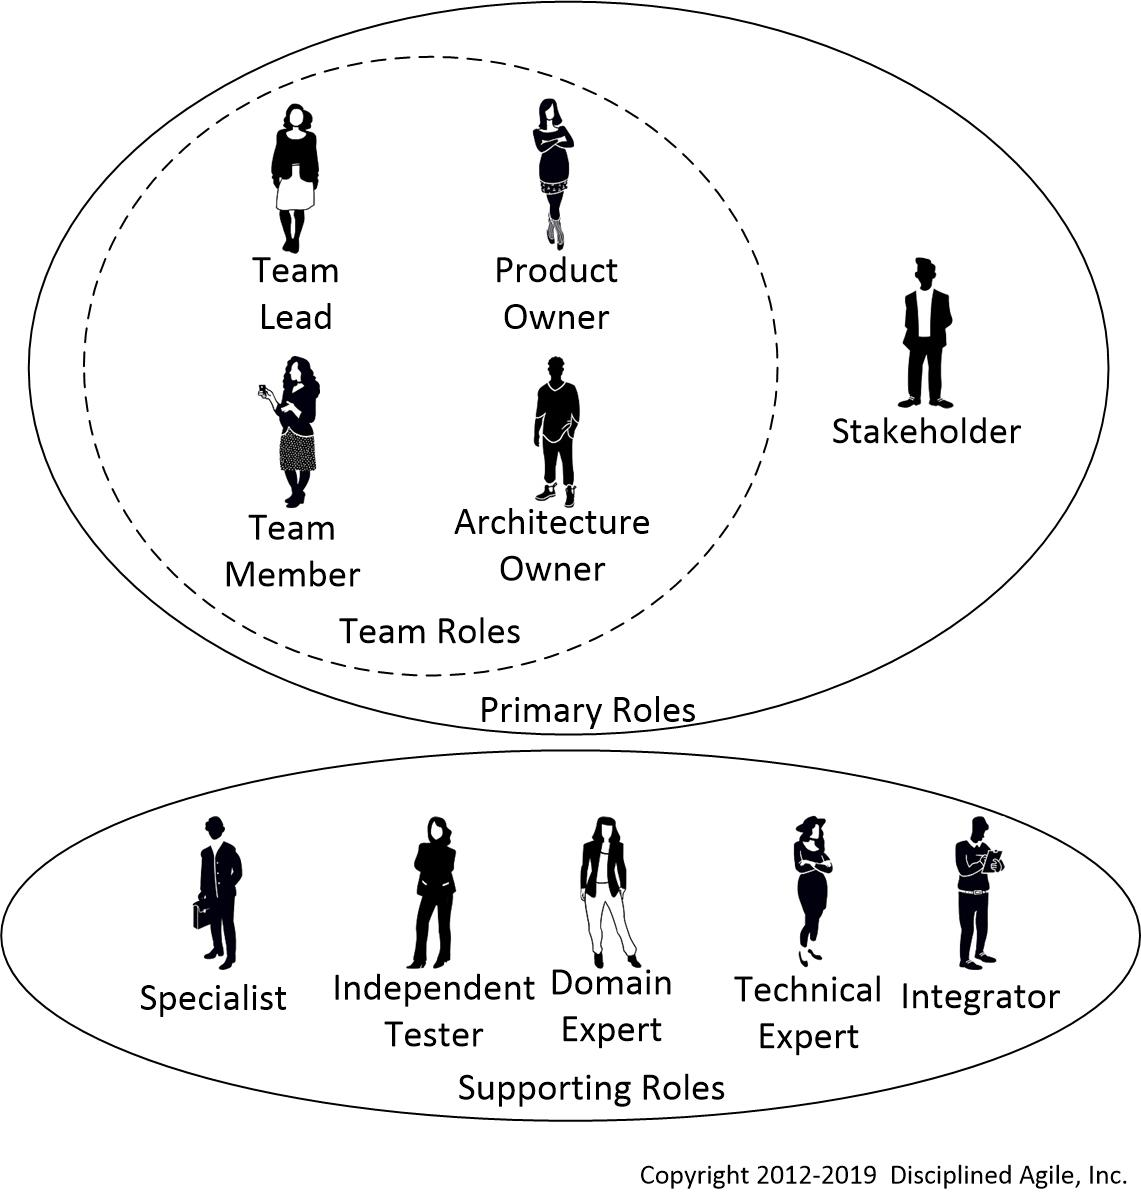
\includegraphics[scale=0.8]{DAD-Roles}
	\caption{DAD Rollen}
	\label{fig:dadrollen}
\end{figure}

DAD wurde somit stark auf die Bedürfnisse von Unternehmen weiterentwickelt um Bedürfnisse aus den bestehenden Firmenstrukturen mit Prozessen, Programmen und Rollen anzuwenden. DAD unterstützt mit den sehr spezifischen Rollen hierarchische Unternehmensstrukturen.
\bigskip 


In diesem Punkt unterscheiden sich die zwei Methoden wesentlich. Warum hat Scrum drei Rollen, DAD hingegen zehn? Scrum konzentriert sich hauptsächlich auf Führungs- und Change-Management-Aspekte während der Konstruktion und hat daher Rollen, die dies widerspiegeln. DAD hingegen konzentriert sich explizit auf den gesamten Delivery Lifecycle und alle Aspekte der Lösungsbereitstellung, einschließlich der technischen Aspekte, die Scrum auslässt. Mit einem größeren Umfang kommen also mehr Rollen hinzu. Weil DAD beispielsweise Fragen der agilen Architektur umfasst, beinhaltet es auch eine Rolle des Architecture Owners. Scrum adressiert keine Architektur und beinhaltet auch keine solche Rolle.

\subsection{Zuständigkeiten}

TODO

\subsection{Verantwortlichkeiten}

In diesem Aspekt wird beschrieben wie die Zuständigkeiten auf die Rollen verteilt sind und welche Zuständigkeiten im Prozess wahrgenommen werden müssen.

{\Large Scrum:} \medskip

In Scrum hat jede Rolle ihre Verantwortlichkeit im Prozess. Der Scrum Master hat in erster Linie die Verantwortung zur Einhaltung des Prozesses und der Scrum Spielregeln. Wie bereits im Kapitel Rollen beschrieben hat er die Verantwortung zur Beseitigung von Hindernissen.

Der Product Owner hat die Verantwortung die Vision und Wünsche des Kunden an das Team weiterzugeben. Er ist die Stimme der Stakeholder und somit verantwortlich dies Bedürfnisse des Kunden zu identifizieren.

Die grösste Verantwortung wird jedoch dem Team zugeteilt. Es legt den Umfang fest, welches es umsetzt - das sogenannte Sprint Goal. Es verpflichtet sich dazu das Sprint Goal umzusetzen. Bei Problemen oder Störungen muss das Team zeitnah mit dem Kunden bzw. mit dem Product Owner in Kontakt treten um gegebenenfalls das Sprint Goal anzupassen. Da das Team selbstorganisiert ist, liegt es in seiner Verantwortung wie das Ziel erreicht wird.

\smallskip
{\Large DAD:} \medskip

TODO 

\subsection{Zielerfüllung}

\medskip
{\Large Scrum:} \medskip

Jedes Artefakt, welches in einer Iteration, in Scrum Sprint genannt, umgesetzt wird, wird durch Akzeptanzkriterien beschrieben. Diese werden zusammen mit oder durch den Kunden definiert. Anhand dieser Akzeptanzkriterien wird ein Artefakt gemessen. Die Akzeptanzkriterien dienen dem Team, nebst einer genauen Beschreibung des Artefakts, zur Erreichung des Sprint Ziels.

In Scrum wird nach jedem Sprint die sogenannte Review gemacht. Hier wird dem Kunden das Produkt bzw. die umgesetzten Artefakte präsentiert. Hier hat der Kunde die Möglichkeit lenkend einzugreifen. Da in Scrum in kurzen Iterationen gearbeitet wird, kann der Kunde schnell und zeitnah Einfluss auf Missverständnisse nehmen.

Das Team definiert zudem die Definition of Done. Die DoD definiert, wann ein Task abgeschlossen ist. Diese müssen nicht zwingend deckend zu den Akzeptanzkriterien sein. Oft hat die DoD umfassendere Punkte wie bspw. Tests, Dokumentation, Review etc.

\medskip
{\Large DAD:} \medskip

Grundsätzlich hat DAD dieselben Mechanismen zur Sicherstellung der Zielerreichung wie Scrum. Nach jeder Iteration wird, wie in Scurm auch, die Iteration zusammengefasst. Den Stakeholdern wird eine Demo der umgesetzten Tasks gezeigt. Es wird entschieden ob man mit dem Vorgehen weitermacht und verbessert den Way of Work.

In DAD wird zudem eine gemeinsame Vision mit den Stakeholdern erstellt. Dies ist ein weiteres Mittel zu Sicherstellung der Zielerreichung.

In DAD besteht jede Phase, Inception, Construction, Transition, aus meheren Goals. Ein Goal kann einmal oder mehrmals durchlaufen werden. Ein Goal besteht aus einem oder mehreren Decision Points.

\begin{figure}[H]
	\centering
	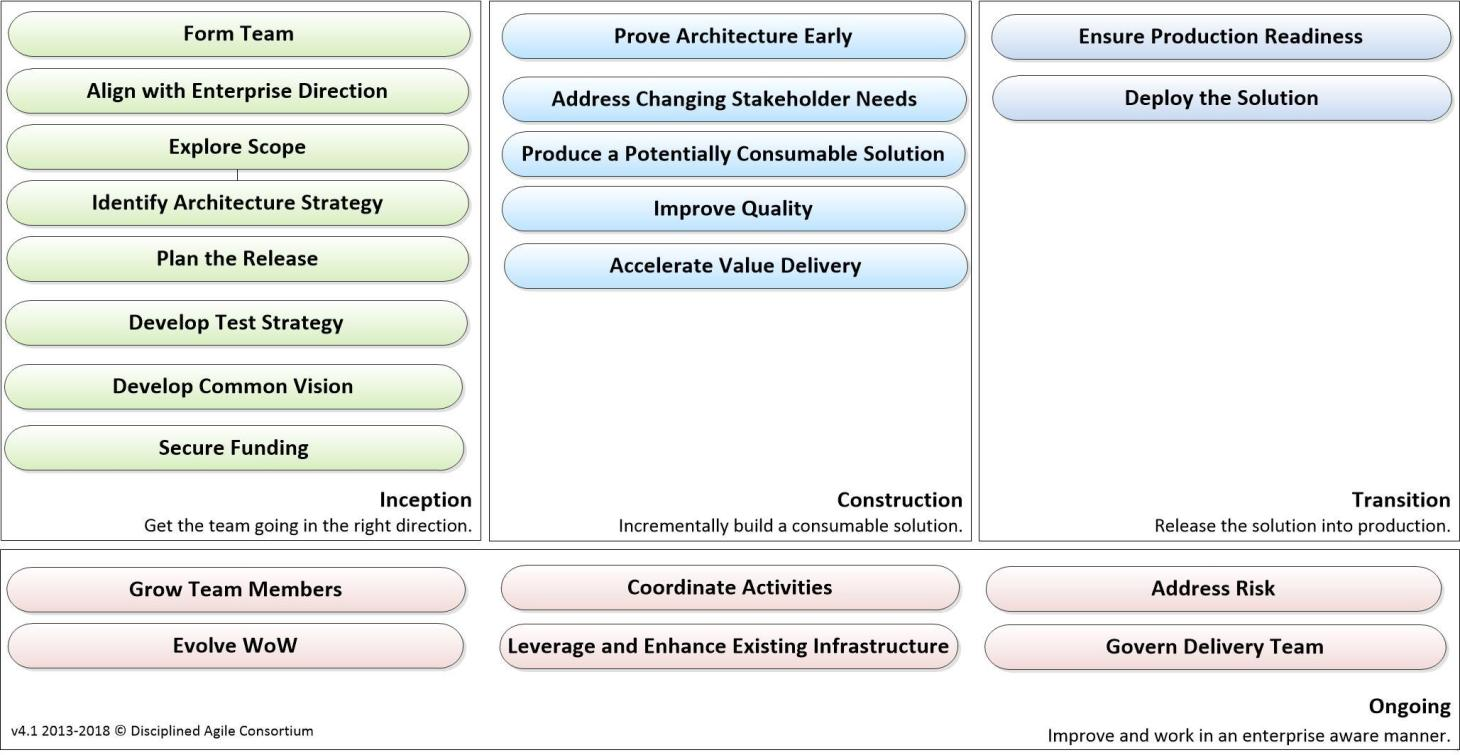
\includegraphics[width=\textwidth]{Lifecycle-Goals.jpg}
	\caption{Lifecycle Goals}
	\label{fig:goals}
\end{figure}

Die Decision Points und Goals dienen der Sicherstellung des Prozesses und somit auch der Erreichung der Ziele.

\subsection{Rollenkonflikte}
TODO
\section{Zusammenarbeit}
TODO


\section{Empfehlung}

Grundsätzlich wäre der Ansatz mit DAD sicher spannend. Ihr Team kann nach wie vor mit Scrum arbeiten und Sie haben die Möglichkeit mit den erwähnten Instrumenten wie leichte Meilensteine, Release Planung der agilen Entwicklung Einfluss zu nehmen und dem ganzen einen ein Rahmen zu geben. \newline
Jedoch wird Sie das Einführen dieses Vorgehensmodell hohen Aufwand kosten. Vor allem muss für das saubere Anwenden von DAD viel Analyse von bestehenden Prozessen und Zuständen innerhalb Ihres Unternehmens betrieben werden.



	